\newpage
\section{Teoria}
\subsection{Osciladores}
Osciladores podem, geralmente, ser categorizados como amplificadores com feedback positivo ou como circuitos de resistência negativa \citep{Rhea}, sendo que nesse experimento são analisado os circuitos com feedback positivo.

\subsection{Ganho do amplificador realimentado}
A figura \ref{f_gain} mostra o diagrama de bloco que representa um amplificador genérico ligado com feedback positivo \citep{abrao, Rhea}.
Neste tipo de amplificador o sinal de entrada $X_s(t)$ é somado ao sinal de saída $X_0(t)$ multiplicado por um ganho $\beta$. Sendo assim, temos que o ganho de transferência do amplificador é 
\[
A_f = \frac{X_0}{X_s} = \frac{A}{1+\beta A}.
\]

Sendo que, segundo \cite{abrao}, para que haja oscilação, o sinal $X_f$ deve estar com uma defasagem de 0 graus em relação a $X_i$. Isto pode ser obtido colocando um bloco de atraso entre $X_s$ e $X_i$.

\begin{figure}[H]
\centering
\caption{Diagrama de blocos de um amplificador com realimentação positiva.}\label{f_gain}
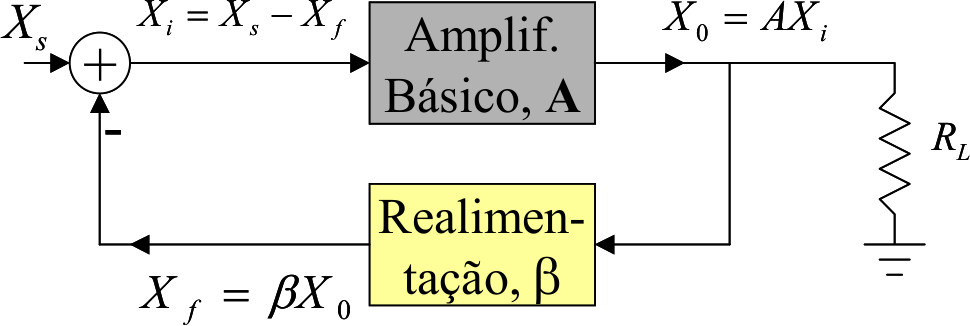
\includegraphics[scale=0.5]{Imagens/gain.png}

\small Fonte: Taufik Abrão, 2002.
\end{figure}

Um outro fator é para que haja oscilação é que $1+A\beta = 0$, ou seja $A\beta = -1$. Como os componentes envolvidos não são ideais, calcula-se o ganho $A\beta$ para valores entre $-1.05$ a $-1.20$ \citep{abrao}.

A frequência de oscilação do circuito (dado que os critérios acima são respeitados) é determinada pela equação \ref{e_freq} \citep{abrao}.

\begin{equation}
f_0 = \frac{1}{2\pi\sqrt{LC}}
\label{e_freq}
\end{equation}
